\documentclass[border=1pt]{standalone}
\usepackage[T1]{fontenc}
\usepackage{mathptmx}
\usepackage{tikz}
\usetikzlibrary{arrows.meta}
\begin{document}
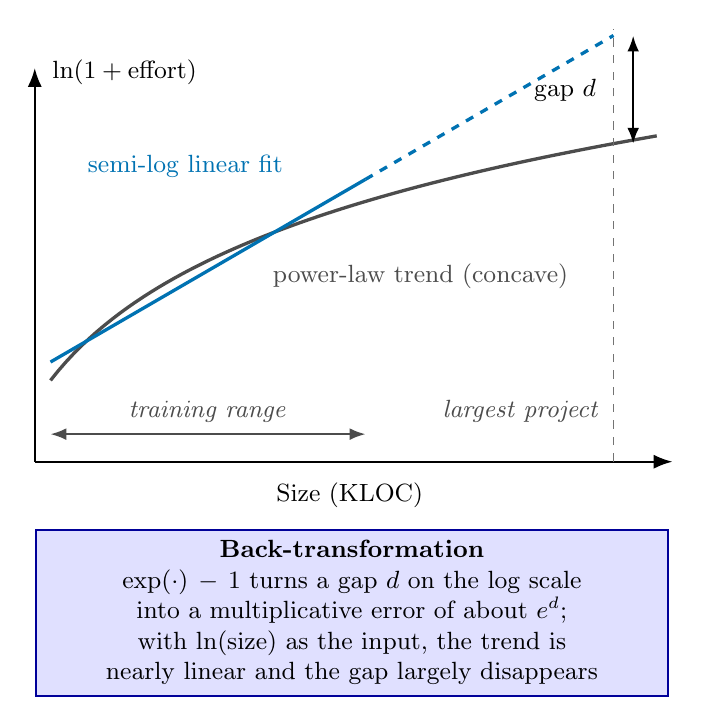
\begin{tikzpicture}[font=\small, x=1cm, y=1cm]
\definecolor{fit}{HTML}{0072B2}
% axes
\draw[-{Latex[length=2.4mm]}, line width=0.8pt] (0,0) -- (0,5.0);
\draw[-{Latex[length=2.4mm]}, line width=0.8pt] (0,0) -- (8.1,0);
\node[anchor=west] at (0.1,4.95) {$\ln(1+\mathrm{effort})$};
\node[anchor=north] at (4.0,-0.15) {Size (KLOC)};
% concave power-law trend: y = 0.75 + 1.55*ln(1+x)
\draw[line width=1.2pt, black!70, domain=0.2:7.9, samples=80] plot (\x,{0.75+1.55*ln(1+\x)});
% linear fit through x=0.75 and x=2.9 on the curve
\draw[line width=1.2pt, fit] (0.2,1.266) -- (4.2,3.586);
\draw[line width=1.2pt, fit, dashed] (4.2,3.586) -- (7.35,5.413);
% largest project
\draw[dashed, black!55, line width=0.7pt] (7.35,0) -- (7.35,5.5);
\draw[{Latex[length=2mm]}-{Latex[length=2mm]}, line width=0.8pt] (7.6,4.04) -- (7.6,5.41);
\node[anchor=east] at (7.25,4.72) {gap $d$};
\node[fit, anchor=west] at (0.55,3.75) {semi-log linear fit};
\node[black!70, anchor=west] at (2.9,2.35) {power-law trend (concave)};
\draw[{Latex[length=2mm]}-{Latex[length=2mm]}, line width=0.7pt, black!70] (0.2,0.35) -- (4.2,0.35);
\node[black!70, anchor=south] at (2.2,0.38) {\emph{training range}};
\node[black!70, anchor=south east] at (7.3,0.38) {\emph{largest project}};
% note
\node[draw=blue!60!black, fill=blue!12, line width=0.7pt, text width=7.75cm, align=center, inner sep=4pt, anchor=north west] at (0,-0.85)
 {\textbf{Back-transformation}\\ $\exp(\cdot)-1$ turns a gap $d$ on the log scale into a \mbox{multiplicative} error of about $e^{d}$; with $\ln(\mathrm{size})$ as the input, the trend is nearly linear and the gap largely disappears};
\end{tikzpicture}
\end{document}
